\documentclass[11pt, twoside]{article}
\usepackage[francais]{babel}
\usepackage[T1]{fontenc}
\usepackage[latin1]{inputenc}
\usepackage[left=5mm, right=5mm, top=3mm, bottom=3mm]{geometry}
\usepackage{float}
\usepackage{graphicx}
\usepackage{array}
\usepackage{multirow}
\usepackage{amsmath,amssymb,mathrsfs}
\usepackage{soul}
\usepackage{textcomp}
\usepackage{eurosym}
 \usepackage{variations}
\usepackage{tabvar}


\pagestyle{empty}

\begin{document}

\begin{center}
\Large{\textbf{Devoir maison 4}}
\end{center}
 

\begin{center}
\fbox{
\begin{minipage}{19cm}
\textit{Devoir � rendre sur feuille grand format pour le
\textbf{mardi 24 f�vrier 2015}. Pensez � bien r�diger. Not� sur 30.}
\end{minipage}
}
\end{center}


\ul{Exercice 1}: (\textit{4 points})



\begin{tabular}{cc}
\begin{minipage}{13cm}
En utilisant les informations de la figure ci-contre, calculer les longueurs BE
et CA.


L'unit� est le centim�tre, la figure n'est pas � l'�chelle.
\end{minipage}

&
\begin{minipage}{5cm}
\begin{center}
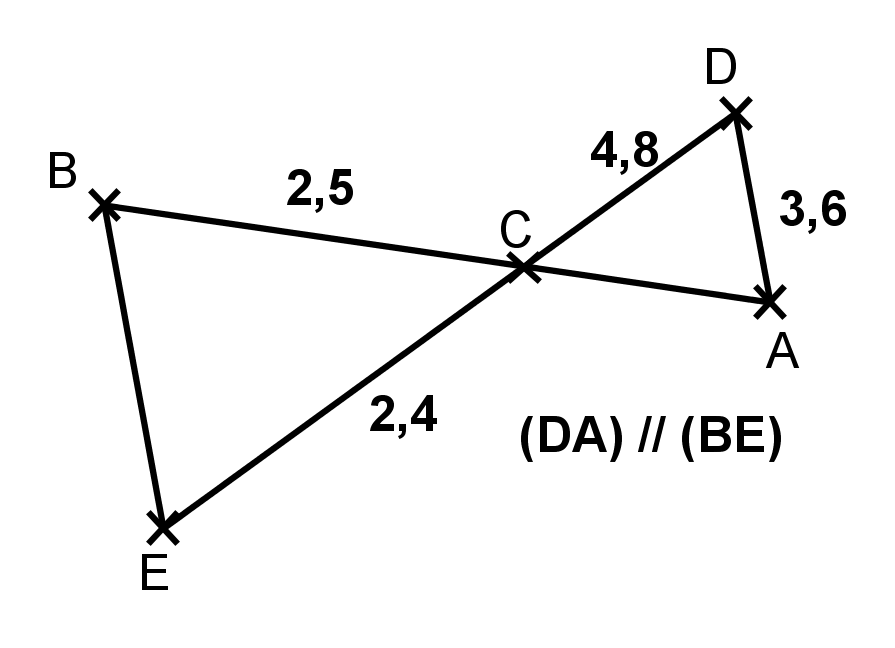
\includegraphics[width=40mm]{images/ex1.png}
\end{center}
\end{minipage} 
\end{tabular}

\enskip

\ul{Exercice 2}: (\textit{6 points})



\begin{tabular}{cc}
\begin{minipage}{15cm}
OAB est un triangle rectangle en A. D appartient � la droite (OB) et C
appartient � la droite (OA). On donne en millim�tres: OC=28; OD=35; CD=21;
OA=42.
\end{minipage}

&
\begin{minipage}{4cm}
\begin{center}
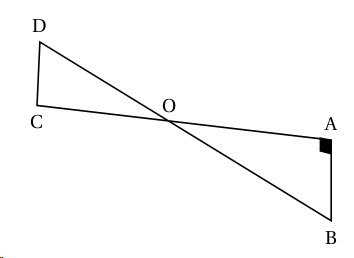
\includegraphics[width=35mm]{images/ex2.jpg}
\end{center}
\end{minipage} 
\end{tabular}


\begin{enumerate}
  \item Montrer que le triangle ODC est rectangle en C.
  \item Que peut-on dire des droites (DC) et (AB)? Justifier votre r�ponse.
  \item Calculer les longueurs OB et AB.
\end{enumerate}

\bigskip

\enskip

\begin{tabular}{cc}
\begin{minipage}{10cm}
\ul{Exercice 3}: (\textit{6,5 points})


\enskip

La figure ci-dessous n'est pas en vraie grandeur. Le quadrilat�re BREV est un
rectangle avec BR=13 cm et BV=7,2 cm. Le point T est sur le segment [VE] tel
que VT=9,6 cm. N est le point d'intersection des droites (BT) et (RE).


\begin{center}
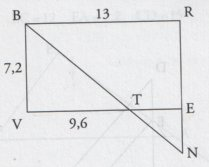
\includegraphics[width=4cm]{images/ex3.jpg}
\end{center}

\begin{enumerate}
  \item Montrer que TE=3,4 cm.
  \item Calculer la longueur BT.
  \item Calculer la longueur EN.
  \item Calculer la longueur TN.
\end{enumerate}

\end{minipage}
&
\begin{minipage}{9cm}


\begin{center}

\ul{Exercice 4:} \textit{(5 points)}

\enskip

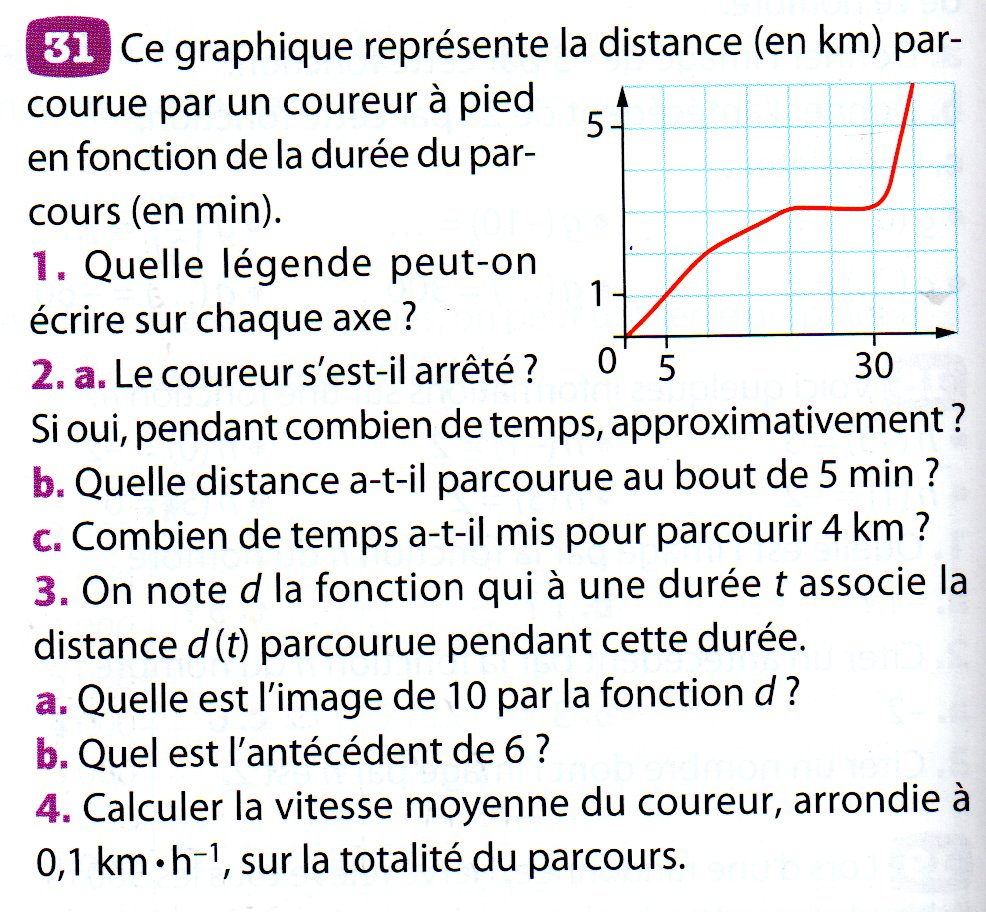
\includegraphics[width=8cm]{images/ex2-fct.jpg}
\end{center}

\end{minipage}
\end{tabular}




\bigskip

\enskip


\begin{tabular}{cc}
\begin{minipage}{9cm}
\ul{Exercice 5:} \textit{(5,5 points)}

\enskip

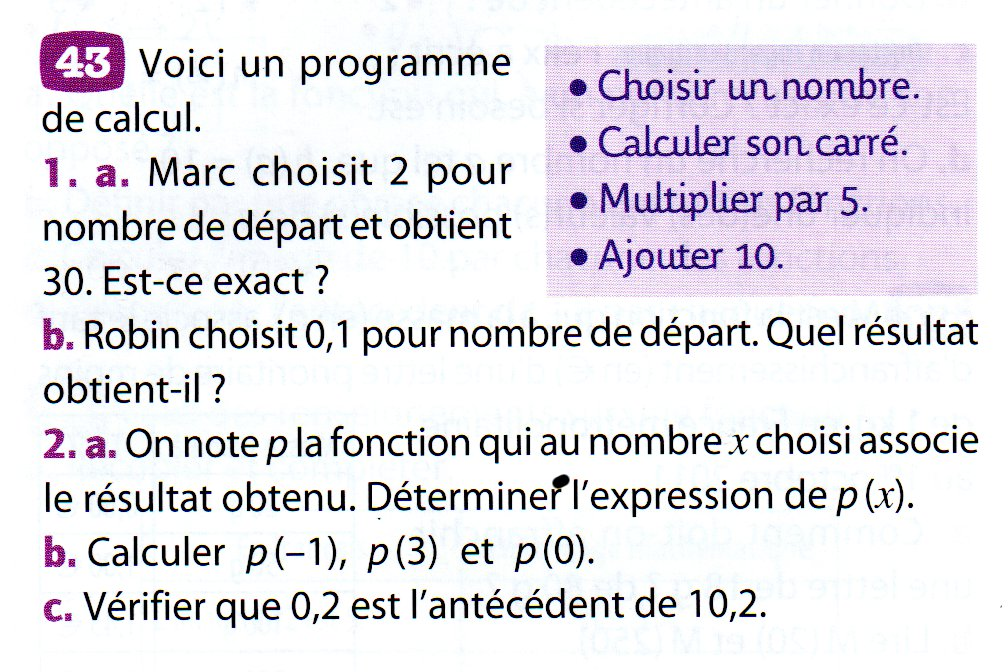
\includegraphics[width=8cm]{images/ex1.jpg}
\end{minipage}
&
\begin{minipage}{9cm}


\begin{center}
\ul{Exercice 6:} \textit{(3 points)}

\enskip

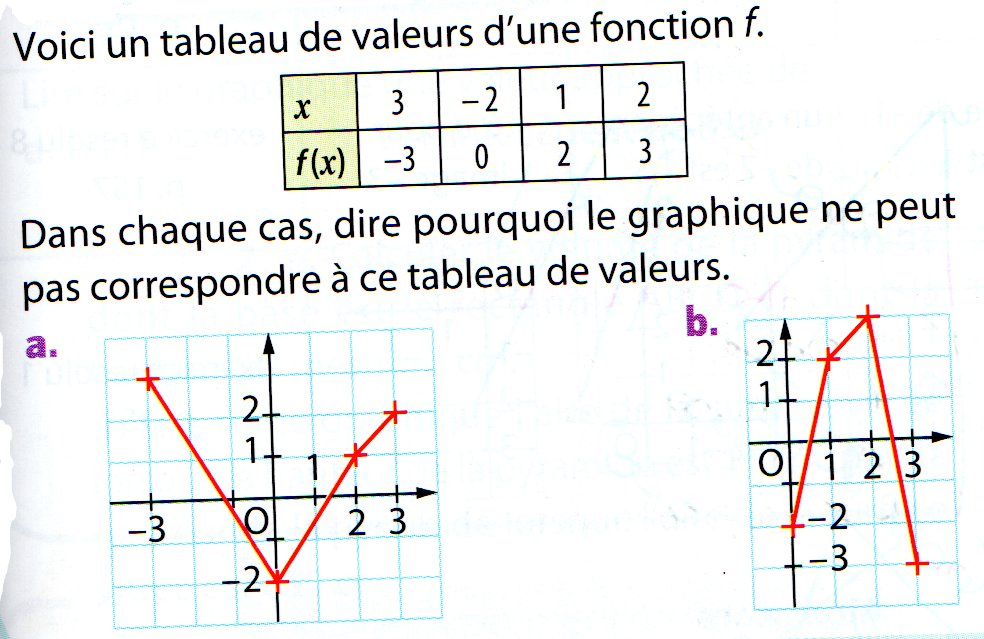
\includegraphics[width=8cm]{images/ex3-fct.jpg}
\end{center}

\end{minipage}


\end{tabular}



\end{document}
